\begin{document}

% Change the following values to true to show the solutions or/and the hints
\ShowSolutiontrue
\ShowConseiltrue
\titre
\cours{Algorithmes de tri et Complexité - exercices basiques}

\begin{enumerate}
    \item la complexité des algorithmes,
    \item la récursivité et
    \item les algorithmes de tri
\end{enumerate}

Les languages de programmation qui seront utilisés pour cette série d'exercices sont Java et Python.


\section{Complexité}

Pour chacun des programmes ci-dessous, donnés à chaque fois en Python et Java, indiquez en une phrase, ce que font ces algorithmes et calculez leur complexité temporelle avec la notation $O( )$. Le code est écrit en Python et en Java. \\

\begin{Exercice}[10 minutes] \textbf{Complexité} \\

    Quelle est la complexité du programme ci-dessous?\\
    \textbf{Python :}
    \begin{lstlisting}{language=Python}
    # Entrée: n un nombre entier
    def algo1(n):
        s = 0
        for i in range(10*n):
            s += i
        return s
    \end{lstlisting}
    
    \textbf{Java :}
    \begin{lstlisting}{language=Java}
        public static int algo1(int n) {
            int s = 0;
            for (int i=0; i < 10*n; i++){
                s += i;
            }
            return s;
        }
    \end{lstlisting}

    \begin{enumerate}
        \item $O(n)$
        \item $O(n^3)$
        \item $O(\log(n))$
        \item $O(n^n)$
    \end{enumerate}
    
    \begin{conseil}
    Rappelez vous que la notation $O()$ sert à exprimer la complexité d'algorithmes dans le \textbf{pire des cas}. Les règles suivantes vous seront utiles. Pour $n$ étant la taille de vos données, on a que :
    \begin{enumerate}
        \item Les constantes sont ignorées : $O(2n) = 2*O(n) = O(n)$ 
        \item Les termes dominés sont ignorés : $O(2n^2+5n+50)$ = $O(n^2)$
    \end{enumerate}
    \end{conseil}

    \begin{solution}
        L'algorithme est composé d'une boucle qui incrémente une variable \lstinline{s}. Il effectue $10*n$ l'opération et par conséquent a une complexité de $O(n)$.
    \end{solution}
\end{Exercice}
\newpage
\begin{Exercice}[10 minutes] \textbf{Complexité} \\
    Quelle est la complexité du programme ci-dessous?\\
    \textbf{Python :}
    \begin{lstlisting}[language=Python]
        # Entrée: L est une liste de nombres entiers et M un nombre entier
        def algo2(L, M):
            i = 0
            while i < len(L) and L[i] <= M:
                i += 1
            s = i - 1
            return s
    \end{lstlisting}
    
    \textbf{Java :}
    \begin{lstlisting}[language=Java]
        public static int algo2(int[] L, int M) {
            int i = 0;
            while (i < L.length && L[i] <= M){
                i += 1;
            }
            int s = i - 1;
            return s;
        }
    \end{lstlisting}

    \begin{enumerate}
        \item $O(n^3)$
        \item $O(\log(n))$
        \item $O(n)$
        \item $O(n^n)$
    \end{enumerate}

    \begin{solution}
    L'algorithme est composé d'une boucle \lstinline{while} qui va parcourir une liste \lstinline{L} jusqu'à trouver une valeur qui est supérieure à \lstinline{M}. Ainsi, dans le pire des cas, l'algorithme parcourt toute la liste, et a donc une complexité de $O(n)$, $n$ étant la taille de la liste.
    \end{solution}
\end{Exercice}
\begin{Exercice}[10 minutes] \textbf{Complexité} \\
    Quelle est la complexité du programme ci-dessous?\\
        \textbf{Python :}
        \begin{lstlisting}[language=Python]
        #Entrée: L et M sont 2 listes de nombre entiers
        def algo3(L, M):
            n = len(L)
            m = len(M)
            for i in range(n):
                L[i] = L[i]*2
            for j in range(m):
                M[j] = M[j]%2
        \end{lstlisting}
        
        \textbf{Java :}
        \begin{lstlisting}[language=Java]
            public static void algo3(int[] L, int[] M) {
                int n = L.length;
                int m = M.length;
                for (int i=0; i < n; i++){
                    L[i] = L[i]*2;
                }
                for (int j=0; j < m; j++){
                    M[j] = M[j]%2;
                }
            }
        \end{lstlisting}

        \begin{enumerate}
            \item $O(n^2)$
            \item $O(n + m)$
            \item $O(n)$
            \item $O(2^n)$
        \end{enumerate}

        \begin{solution}
        L'algorithme est composé de 2 boucles. La première parcourt une liste \lstinline{L} et multiplie par 2 les éléments de la liste. 
        L'autre parcourt une liste \lstinline{M} et assigne à chaque élément le reste de la division euclidienne de l'élément par 2. 
        Soient $n$ et $m$ les tailles respectives de \lstinline{L} et de \lstinline{M}, on obtient une complexité de $O(n + m)$. 
        Ainsi, l'élément ayant la plus grande complexité sera utilisé pour déterminer la complexité de l'algorithme dans son ensemble.
        \end{solution}
\end{Exercice}

\begin{Exercice}[10 minutes] \textbf{Complexité} \\
    Quelle est la complexité du programme ci-dessous?\\
    \textbf{Python :}
    \begin{lstlisting}[language=Python]
    #Entrée: L est une liste de nombre entiers
    def algo4(L):
        n = len(L)
        i = 0
        s = 0
        while i < math.log(n):
            s += L[i]
            i += 1
        return s
    \end{lstlisting}
    
    \textbf{Java :}
    \begin{lstlisting}[language=Java]
        import java.lang.Math; 

        public static void algo4(int[] L) {
            int n = L.length;
            int s = 0;
            for (int i=0; i < Math.log(n); i++){
                s += L[i];
            }
        }
    \end{lstlisting}

    \begin{enumerate}
        \item $O(n^2)$
        \item $O(n)$
        \item $O(\log(n))$
        \item $O(n^n)$
    \end{enumerate}

    \begin{solution}
    L'algorithme est composé d'une boucle qui va itérer sur $\log(n)$ éléments et 
    va calculer la somme de ces éléments. Ainsi, l'algorithme a une complexité de $O(\log n)$.
    Le temps d'exécution de ce programme peut être visualisé sur la courbe jaune du graphe ci-dessous (\ref{bigO}).
    \end{solution}
    
    \begin{figure}[h!]
        \centering
        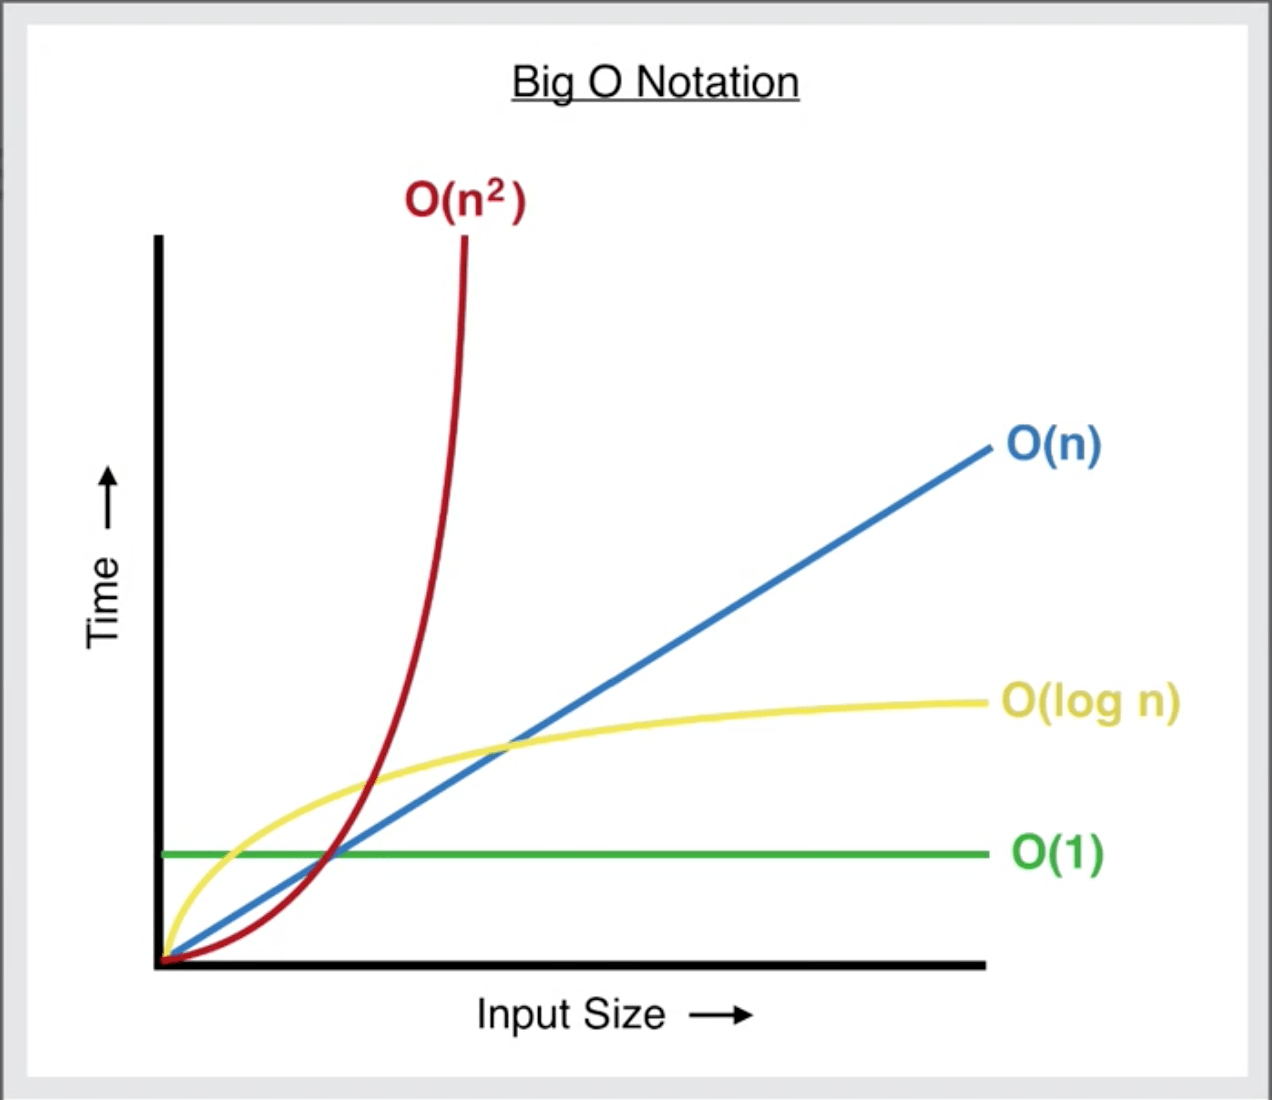
\includegraphics[width=10cm]{ressources/complexity.png}
        \caption{Représentation de complexités temporelles}
        \label{bigO}
    \end{figure}

    

\end{Exercice}

\newpage

\begin{Exercice}[10 minutes] \textbf{Complexité} \\
    Quelle est la complexité du programme ci-dessous?\\
        \textbf{Python :}
        \begin{lstlisting}[language=Python]
        # Entrée: n un nombre entier
        def algo5(n):
            m = 0
            for i in range(n):
                for j in range(i):
                    m += i+j
            return m
        \end{lstlisting}
        
        \textbf{Java :}
        \begin{lstlisting}[language=Java]
            public static int algo5(int n) {
                int m = 0;
                for (int i=0; i < n; i++){
                    for (int j=0; j < i; j++){
                        m += i+j;
                    }
                }
                return m;
            }
        \end{lstlisting}
    
        \begin{enumerate}
            \item $O(n^2)$
            \item $O(n)$
            \item $O(\log(n))$
            \item $O(2^n)$
        \end{enumerate}

    \begin{solution} 
    L'algorithme est composé de 2 boucles \textbf{imbriquées} suivant une suite définie par $\frac{n(n-1)}{2}$. L'algorithme va additionner les index $i$ et $j$ à chaque itération et les rajouter à $m$.
    Cela veut dire que nous parcourons la liste un maximum de $n \times n$ fois, $n$ étant la taille de la liste. La complexité de l'algorithme est ainsi de $O(n^2)$.
    \end{solution}
    
\end{Exercice}
    
        
\section{Récursivité}

Le but principal de la récursivité est de résoudre un gros problème en le divisant en plusieurs petites parties à résoudre.


\begin{Exercice} [10 minutes] \textbf{Fibonacci}\\
La suite de Fibonacci est définie récursivement par les propriétés suivantes:
\begin{itemize}
    \item si n est égal à 0 ou 1 : fibo(0) = fibo(1) = 1
    \item si n est supérieur ou égal à 2, alors ; fibo (n) = fibo(n - 1) + fibo(n - 2)
\end{itemize}

Voici son implémentation en Java :

\begin{lstlisting}{language=Java}
        public static int fibonacci(int n) {
            if(n == 0 | n == 1){
                return n;
            } else{
                return fibonacci(n-1) + fibonacci(n-2);
            }
        }
        
\end{lstlisting}

Quel est la complexité de l'algorithme ci-dessus?

\begin{note}{Arnaud}
    Peut-être faire la correction en commun pour la démonstration de T(n)=(2^k)*T(n-k)+((2^k)-1)
\end{note}

\begin{conseil}
Aidez-vous d'un exemple (\lstinline{fibonacci(3)}, \lstinline{fibonacci(4)},...) \\
Pour formaliser la formule de complexité, on peut poser que $T(n)$ énumère le nombre d'opérations requises pour calculer \lstinline{fibonacci(n)}. Ainsi, $T(n) = T(n-1) + T(n-2) + c$, $c$ étant une constante. Vous pouvez alors énumérer le nombre d'opérations pour \lstinline{fibonacci(3)}, \lstinline{fibonacci(4)}... et esssayer de trouver la complexité en terme de $O()$.
\end{conseil}

\ \\

\begin{enumerate}
    \item $O(n^2)$
    \item $O(n)$
    \item $O(\log(n))$
    \item $O(2^n)$
\end{enumerate}

\begin{solution}
    La complexité de cet algorithme est $O(2^n)$.
\end{solution}
\end{Exercice}

\section{Algorithmes de Tri}

\begin{Exercice} [20 minutes] \textbf{Tri à bulles (Bubble Sort) en python} \\
Le tri à bulles consiste à parcourir une liste et à comparer ses éléments. Le tri est effectué en permutant les éléments de telle sorte que les éléments les plus grands soient placés à la fin de la liste. 

Concrètement, si un premier nombre $x$ est plus grand qu'un deuxième nombre $y$ et que l'on souhaite trier l'ensemble par ordre croissant, alors $x$ et $y$ sont mal placés et il faut les inverser. Si, au contraire, $x$ est plus petit que $y$, alors on ne fait rien et l'on compare $y$ à $z$, l'élément suivant.

Soit la liste \lstinline{l = [1, 2, 4, 3, 1]}, triez les éléments de la liste en utilisant un tri à bulles. Combien d'itérations effectuez-vous?

\begin{itemize}
        \item \textbf{Python :}
            \lstinputlisting{ressources/question8.py} 
    \end{itemize}
    
    \ \\
    
    \begin{solution}
    \textbf{Python :}
    \lstinputlisting{solutions/question8.py}

    L'algorithme a une complexité de $O(n^2)$ car il contient deux boucles qui parcourent la liste.\\\\\\
            
\end{solution}
\end{Exercice}

\begin{Exercice}[10 minutes] \textbf{Tri par insertion - 1 (Python)}\\
    Soit un nombre entier \lstinline{n}, et une liste triée \lstinline{l}. Ecrivez un programme Python qui insère la valeur \lstinline{n} dans la liste \lstinline{l} tout en s'assurant que la liste \lstinline{l} reste triée.

    \lstinputlisting{ressources/question9.py}

    \begin{Exemple}{\faTerminal \quad Exemple}
        En passant les arguments suivants à votre programme: n=5 et l=[2,4,6]. Ce dernier devra retourner \lstinline{l =[2,4,5,6]}
    \end{Exemple}

    \begin{solution}
        \lstinputlisting{solutions/question9.py}
    \end{solution}


\end{Exercice}

\begin{Exercice} [20 minutes] \textbf{Tri par insertion - 2 (Insertion Sort)} \\

    Dans l'algorithme de tri par insertion, on parcourt le tableau à trier du début à la fin. Au moment où on considère le i-ème élément, les éléments qui le précèdent sont déjà triés. Pour faire l'analogie avec l'exemple du jeu de cartes, lorsqu'on est à la i-ème étape du parcours, le i-ème élément est la carte saisie, les éléments précédents sont la main triée et les éléments suivants correspondent aux cartes encore en désordre sur la table. 
    
    L'objectif d'une étape est d'insérer le i-ème élément à sa place parmi ceux qui le précède. Il faut pour cela trouver où l'élément doit être inséré en le comparant aux autres, puis décaler les éléments afin de pouvoir effectuer l'insertion. En pratique, ces deux actions sont fréquemment effectuées en une passe, qui consiste à faire ``remonter'' l'élément au fur et à mesure jusqu'à rencontrer un élément plus petit. 
    
    Compléter le code suivant pour trier la liste \lstinline{l} définie ci-dessous en utilisant un tri par insertion. Combien d'itérations effectuez-vous?
    \begin{itemize}
        \item \textbf{Python :}
            \lstinputlisting{ressources/question10.py} 
        \item \textbf{Java :}
            \lstinputlisting{ressources/question10.java} 
    \end{itemize}
    
    \begin{conseil}
        Référez vous à la figure du dessous pour un exemple de tri par insertion. \\
        Référez vous aussi aux diapositives 18 à 72 du cours.
    \end{conseil}
    
    \begin{figure}[h!]
        \centering
        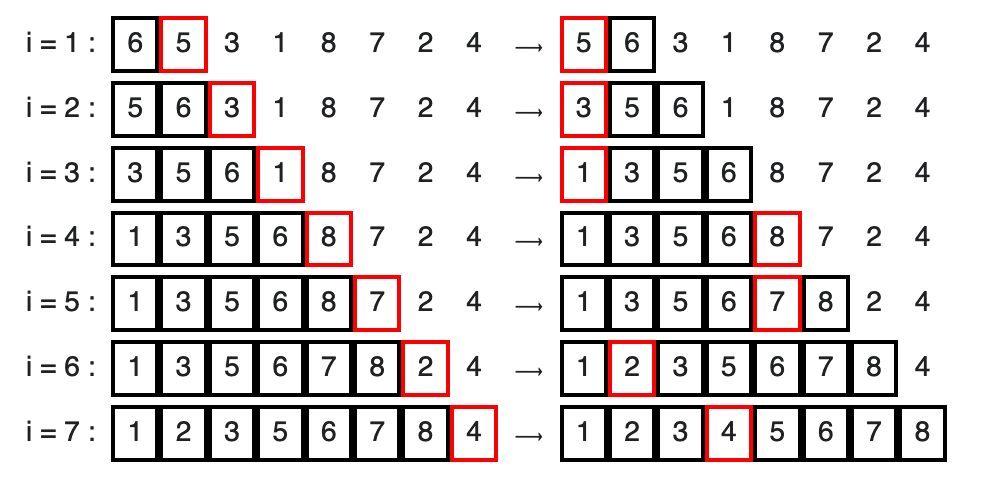
\includegraphics[width=10cm]{ressources/tri_insertion.png}
    \end{figure}

    \begin{solution}
        \textbf{Python :}
            \lstinputlisting{solutions/question10.py} 
        \textbf{Java :}
            \lstinputlisting{solutions/question10.java}
    
    La complexité de l'algorithme est de $O(n^2)$ car nous utilisons 2 boucles imbriquées, qui dans le pire des cas, parcourent la liste deux fois.
    \end{solution}
    
\end{Exercice}

\begin{Exercice} [20 minutes] \textbf{Tri fusion (Merge Sort) en python} \\
    À partir de deux listes triées, on peut facilement construire une liste triée comportant les éléments issus de ces deux listes (leur \textit{fusion}). Le principe de l'algorithme de tri fusion repose sur cette observation : le plus petit élément de la liste à construire est soit le plus petit élément de la première liste, soit le plus petit élément de la deuxième liste. Ainsi, on peut construire la liste élément par élément en retirant tantôt le premier élément de la première liste, tantôt le premier élément de la deuxième liste (en fait, le plus petit des deux, à supposer qu'aucune des deux listes ne soit vide, sinon la réponse est immédiate). 
    
    Les étapes à suivre pour implémenter l'algorithme sont les suivantes:
    \begin{enumerate}
        \item Si le tableau n'a qu'un élément, il est déjà trié.
        \item Sinon, séparer le tableau en deux parties plus ou moins égales.
        \item Trier récursivement les deux parties avec l'algorithme de tri fusion.
        \item Fusionner les deux tableaux triés en un seul tableau trié.
    \end{enumerate}
    
    Soit la liste \lstinline{l} suivante [38, 27, 43, 3, 9, 82, 10], triez les éléments de la liste en utilisant un tri fusion. Combien d'itération effectuez-vous?
    
    \begin{itemize}
        \item \textbf{Python :}
            \lstinputlisting{ressources/question11.py}
    \end{itemize}
    
    \begin{conseil}
    \begin{itemize}
        \item L'algorithme est récursif. 
        \item Revenez à la visualisation de l'algorithme dans les diapositives 83 à 111 pour comprendre comment marche concrètement le tri fusion. 
    \end{itemize}
    
    \end{conseil}
    
    \begin{solution}
        \textbf{Python :}
         \lstinputlisting{solutions/question11.py}
    \end{solution}
\end{Exercice}


\end{document}
